\documentclass[usenames,dvipsnames, 9pt]{beamer}
\usepackage{amsmath,amsfonts,amssymb}
\usepackage{mathtools}
\usepackage{etex} %for Windows
\usepackage[utf8]{inputenc}
\usepackage[english, russian]{babel} 
%\usepackage{microtype}			% Better interword spacing and additional kerning.
\usepackage{ellipsis}			% Adjusted space with \dots between two words.
\usepackage{graphicx}
\usepackage{pstricks}

\usepackage{xcolor}


\usepackage{changepage}

\usepackage{algorithm}
\usepackage{algpseudocode}
%\usepackage[]{algorithm2e}
%\usepackage{algorithmic}

%\usepackage{tcolorbox}


\usepackage{caption}
\usepackage{subcaption}
%\usepackage{stackengine}


\usepackage{tikz}
\usetikzlibrary{tikzmark,calc}
\usetikzlibrary{positioning, backgrounds}
\usetikzlibrary{arrows, chains, matrix, scopes, patterns, shapes, fit}
\usetikzlibrary{mindmap,trees,shadows}
\usetikzlibrary{decorations.pathreplacing}
%\usetikzlibrary{crypto.symbols}

\usepackage{pgfplots}

\pgfmathdeclarefunction{gauss}{2}{%
	\pgfmathparse{1/(#2*sqrt(2*pi))*exp(-((x-#1)^2)/(2*#2^2))}%
}


\tikzset{
	invisible/.style={opacity=0},
	visible on/.style={alt={#1{}{invisible}}},
	alt/.code args={<#1>#2#3}{%
		\alt<#1>{\pgfkeysalso{#2}}{\pgfkeysalso{#3}} % \pgfkeysalso doesn't change the path
	},
}

\newcommand\strikeout[2][]{%
	\begin{tabular}[b]{@{}c@{}} 
		\makebox(0,0)[cb]{{#1}} \\[-0.2\normalbaselineskip]
		\rlap{\color{Orange}\rule[0.5ex]{\widthof{#2}}{1.5pt}}#2
\end{tabular}}

\newcommand\Fontvi{\fontsize{11}{13.2}\selectfont}

\usepackage{listings} % for C++ code

\usepackage{braket}
%\usepackage[braket, qm]{qcircuit}



\usepackage[T1]{fontenc}
%\usepackage[sfdefault,scaled=.85]{FiraSans}
%\usepackage{newtxsf}
%\usepackage[nomap]{FiraMono}





\usefonttheme[onlymath]{serif}
\renewcommand\sfdefault{cmbr}

\renewcommand{\bfdefault}{sb}

\definecolor{CharCoalDark}{RGB}{13, 16, 19}
\definecolor{Orange}{RGB}{255, 165,0}
\definecolor{DarkOrange}{RGB}{255, 165,0}
\definecolor{LightSalmon}{RGB}{255, 160, 122}
\definecolor{LeafGreen}{RGB}{34, 139,  34}
\definecolor{Coral}{RGB}{255, 127, 80}
\definecolor{DarkTurquoise}{RGB}{0, 206, 209}

%\newtheorem{defRus}{Определение}
%\newtheorem{thmRus}{Теорема}
%s\newtheorem{corRus}{Следствие}


\setbeamercolor{background canvas}{bg=CharCoalDark}

\setbeamerfont{title}{series=\bfseries}
\setbeamercolor{title}{fg=Orange}
\setbeamercolor{section in toc}{fg=white}
\setbeamercolor{frametitle}{fg=Orange}
\setbeamercolor{normal text}{fg=white}
%\setbeamercolor{normal text}{fontsize=12pt}
\setbeamercolor{itemize item}{fg=Orange}
\setbeamercolor{enumerate item}{fg=Orange}
\setbeamercolor{enumerate item item}{fg=Orange}
\setbeamercolor{itemize item item}{fg=Orange}
\setbeamercolor{enumerate item}{fg=Orange}
\setbeamercolor{block title}{bg=DarkOrange,fg=white}
\setbeamerfont{block title}{series=\bfseries}

\setbeamertemplate{itemize item}[circle]
\setbeamertemplate{eumerate subitem}{\color{Orange}[$\checkmark$]}
\setbeamertemplate{itemize subitem}{\color{Orange}\Large$\textbullet$}
\setbeamertemplate{itemize subitem}{\color{Orange} \tiny $\blacksquare$}

% footnote without a marker
\newcommand\blfootnote[1]{%
	\begingroup
	\renewcommand\footnoterule{}
	\renewcommand\thefootnote{}\footnote{#1}%
	\addtocounter{footnote}{-1}%
	\endgroup
}

\newcommand*{\Scale}[2][4]{\scalebox{#1}{\ensuremath{#2}}}%

\newcommand\Item[1][]{%
	\ifx\relax#1\relax  \item \else \item[#1] \fi
	\abovedisplayskip=0pt\abovedisplayshortskip=0pt~\vspace*{-\baselineskip}}

\pgfdeclareradialshading{ring}{\pgfpoint{0cm}{0cm}}%
{rgb(0cm)=(1,1,1);
	rgb(0.7cm)=(1,1,1);
	rgb(0.719cm)=(1,1,1);
	rgb(0.72cm)=(0.975,0,0);
	rgb(0.9cm)=(1,1,1)}

\usepackage[absolute,overlay]{textpos} %to clip to a corner
\newcommand\FrameText[1]{%
	\begin{textblock*}{\paperwidth}(\textwidth-35pt, 10 pt)
		\raggedright #1\hspace{.5em}
\end{textblock*}}

\makeatletter
\let\save@measuring@true\measuring@true
\def\measuring@true{%
	\save@measuring@true
	\def\beamer@sortzero##1{\beamer@ifnextcharospec{\beamer@sortzeroread{##1}}{}}%
	\def\beamer@sortzeroread##1<##2>{}%
	\def\beamer@finalnospec{}%
}
\makeatother

\AtBeginSection[]
{
	\begin{frame}<beamer>
		\frametitle{Outline}
		\tableofcontents[currentsection]
	\end{frame}
}


%\institute{ENS Lyon}
\author{Elena Kirshanova \\ [10pt]
}
\titlegraphic{
	
	%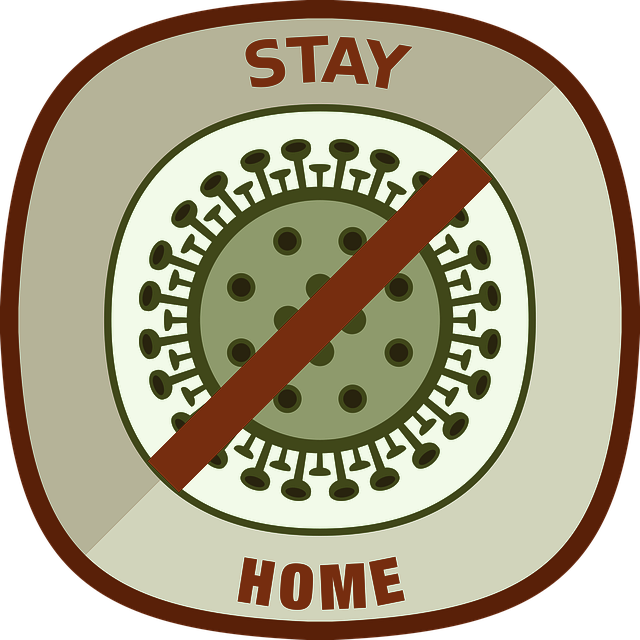
\includegraphics[width=2.5cm]{stayhome}%
	%\includegraphics[width=4.0cm]{ens_logo_gray}
}
\title{\Huge Cryptographic Signature Scheme}

\date{ Course ``Information and Network Security'' \\ 	
	Lecture 9 \\ \today }


\setbeamertemplate{navigation symbols}{} %removes navigation

% proper highlightling of a code-snippet
\lstset{language=C++,
	keywordstyle=\color{magenta},
	stringstyle=\color{Goldenrod},
	commentstyle=\color{gray},
	breaklines=false,
	%morecomment=[l][\color{magenta}]{\#}
}

%\setlength{\parskip}{8pt}
% ==================================================================
% Definitions for this paper
% ==================================================================
\mathchardef\hyphen="2D

\usepackage{multirow}
\usepackage{multicol} % For multiple coloumn environments
%\usepackage{stmaryrd} % For set brackets
% \setlength{\columnsep}{15pt} % Defining the coloumn seperation
% \setlength{\columnseprule}{1pt} % Place a line between coloumns
% \newcommand{\tab}{\hspace*{2em}}

%subscripts

\newcommand*\SmallTextScript[2]{{\mathchoice{\displaystyle #2}
		{\textstyle #2}%dito
		{\scalebox{#1}{\ensuremath{\scriptstyle #2}}}%
		{\scalebox{#1}{\ensuremath{\scriptscriptstyle #2}}}%
}}


% ADVERSARIES AND SUCH
\newcommand*{\poly}{\ensuremath{\mathrm{poly}}}
\newcommand*{\eps}{\ensuremath{\varepsilon}}
\newcommand*{\alg}{\ensuremath{\mathcal{A}}}

% GROUPS/DISTRIBUTIONS/SETS/LISTS
\newcommand{\N}{{{\mathbb N}}}
\newcommand{\Z}{{{\mathbb Z}}}
\newcommand*{\IZ}{\ensuremath{\mathbb{Z}}}
\newcommand*{\IN}{\ensuremath{\mathbb{N}}}
\newcommand*{\IQ}{\ensuremath{\mathbb{Q}}}
\newcommand{\R}{{{\mathbb R}}}
\newcommand*{\IR}{{{\mathbb R}}}
\newcommand{\Zp}{\Z_p} % Integers modulo p
\newcommand{\Zq}{\Z_qs} % Integers modulo q
\newcommand{\Zn}{\ints_N} % Integers modulo N
\newcommand{\F}{\ensuremath{\mathbb{F}}}
\newcommand{\CC}{\ensuremath{\mathbb{C}}}

\newcommand{\ord}{\ensuremath{\mathrm{ord}}}

\newcommand{\GF}{\ensuremath{\mathbb{F}_2}}
\newcommand{\GFn}{\ensuremath{\mathbb{F}^n_2}}

%%% ALGORITHMS/PROCEDURES %%%
\newcommand{\Dec}{\textsf{Dec}}
\newcommand{\Enc}{\textsf{Enc}}
\newcommand{\KeyGen}{\textsf{KeyGen}}
\newcommand{\Gen}{\textsf{Gen}}
\newcommand{\MAC}{\textsf{MAC}}
\newcommand{\sk}{\textsf{sk}}
\newcommand{\pk}{\textsf{pk}}
\newcommand{\mesS}{\ensuremath{\mathcal{M}}}
\newcommand{\keyS}{\ensuremath{\mathcal{K}}}
\newcommand{\cipS}{\ensuremath{\mathcal{C}}}
\newcommand{\tagS}{\ensuremath{\mathcal{T}}}
\newcommand{\nonceS}{\ensuremath{\mathcal{N}}}
\newcommand{\mactag}{\textsf{tag}}
\newcommand{\Hash}{\ensuremath{\mathcal{H}}}
\newcommand{\EID}{\ensuremath{\mathtt{EphID}}}

\newcommand{\rem}{\ensuremath{\mathrm{rem}}}

\newcommand{\adv}{\ensuremath{\mathcal{A}}}

\newcommand{\LWE}{\mathsf{LWE}}
\newcommand{\DCP}{\mathsf{DCP}}
\newcommand{\EDCP}{\mathsf{EDCP}}
\newcommand{\UEDCP}{\mathsf{U \text{-} EDCP}}
\newcommand{\GEDCP}{\mathsf{G \text{-} EDCP}}



%% Landau and proba
\newcommand{\bigO}{\mathcal{O}}
\newcommand*{\OLandau}{\bigO}
\newcommand*{\WLandau}{\Omega}
\newcommand*{\xOLandau}{\widetilde{\OLandau}}
\newcommand*{\xWLandau}{\widetilde{\WLandau}}
\newcommand*{\TLandau}{\Theta}
\newcommand*{\xTLandau}{\widetilde{\TLandau}}
\newcommand{\smallo}{o} %technically, an omicron
\newcommand{\wLandau}{\omega}
\newcommand{\negl}{\mathrm{negl}}
\newcommand*\PROB\Pr 
\DeclareMathOperator*{\EXPECT}{\mathbb{E}}
\DeclareMathOperator*{\VARIANCE}{\mathbb{V}}
\DeclareMathOperator*{\LOGBIAS}{\mathbb{LB}}

\newcommand{\supp}{\ensuremath{\mathsf{sup}}}
\newcommand{\Distr}{\ensuremath{\mathcal{D}}}

% Lattices

% \newcommand{\coset}{\Lambda} % Lambda Lattice
% \newcommand{\cosetPerp}{\Lambda^{\bot}} % Lambda_Perp Lattice
% \newcommand{\gadget}{\textbf{G}} %Gaget matrix
% \newcommand{\mes}{\textbf{m}} %message vector
% \newcommand{\AMat}{\textbf{A}} %A matrices
% \newcommand{\BMat}{\textbf{B}} %B matrices
% \newcommand{\RMat}{\textbf{R}} %R matrices
% \newcommand{\HMat}{\textbf{H}} %H matrices
% \newcommand{\XMat}{\textbf{X}} %H matrices
% \newcommand{\mbar}{\bar{m}} %mBar dimension
% % \newcommand{\gauss}{\mathcal{D}} % gaussian distribution
% \newcommand{\Id}{\textbf{I}} % Identity matrix
% \newcommand{\er}{\textbf{e}} % gaussian distr. vectors
% % \newcommand{\cipher}{\textit{c}} % ciphertext
% \newcommand{\Olwe}{\mathcal{O}_{\textsf{LWE}}} %LWE oracle
% \newcommand{\OSample}{\mathcal{O}_{Sample}} %LWE oracle
% \newcommand{\SigmaB}{\boldsymbol{\Sigma}} %semi-deifinite matrix Sigma%
% % \newcommand{\mods}{\text{ mod}}


%Vectors and Matrices

\newcommand{\AMat}{\mathbf{A}} %A matrices
\newcommand{\BMat}{\mathbf{B}} %B matrices
\newcommand{\DMat}{\mathbf{D}} %Diagonal


\newcommand{\HMat}{\ensuremath{\mathbf{H}}}
\newcommand{\QMat}{\ensuremath{\mathbf{Q}}}
\newcommand{\Id}{\ensuremath{\mathbf{I}}}
\newcommand{\ZeroM}{\textbf{0}} % Zero matrix

\newcommand{\avec}{\ensuremath{\mathbf{a}}}
\newcommand{\bvec}{\ensuremath{\mathbf{b}}}
\newcommand{\cvec}{\ensuremath{\mathbf{c}}}
\newcommand{\evec}{\ensuremath{\mathbf{e}}}
\newcommand{\rvec}{\ensuremath{\mathbf{r}}}
\newcommand{\svec}{\ensuremath{\mathbf{s}}}
\newcommand{\tvec}{\ensuremath{\mathbf{t}}}
\newcommand{\vvec}{\ensuremath{\mathbf{v}}}
\newcommand{\zvec}{\ensuremath{\mathbf{z}}}
\newcommand{\xvec}{\ensuremath{\mathbf{x}}}
\newcommand{\yvec}{\ensuremath{\mathbf{y}}}
\newcommand{\uvec}{\ensuremath{\mathbf{u}}}
\newcommand{\zerovec}{\ensuremath{\mathbf{0}}}

\newcommand{\nth}{^{\mathrm{th}}}
\newcommand{\nd}{^{\mathrm{nd}}}

\newcommand{\RepMMT}{\ensuremath{\mathcal{R}_{\protect\SmallTextScript{0.70}{\texttt{MMT}}}}}
\newcommand{\RepBJMM}{\ensuremath{\mathcal{R}_{\protect\SmallTextScript{0.70}{\texttt{BJMM}}}}}
\newcommand{\XOR}{\ensuremath{\mathtt{3XOR}}}


% % % % % \newcommand{\mb}[1]{\mathbf{#1}} % does not compile otherwise
%%% Removed by Gotti; this is just asking to screw up with packages that (properly) define \mb (mathbold)

% \newcommand{\bL}{\|\bvec_1\|} % b1 length that appears way too often
% \newcommand{\dL}{\|\dvec_1\|} % b1 length that appears way too oftend

%Norms and Scalar products

\newcommand*\abs[1]{\left\lvert#1\right\rvert}
\newcommand*\norm[1]{\left\lVert#1\right\rVert}
\newcommand*\normalabs[1]{\lvert#1\rvert} 
\newcommand*\normalnorm[1]{\lVert#1\rVert}
\newcommand*\bignorm[1]{\bigl\lVert#1\bigr\rVert}
\newcommand*\bigabs[1]{\bigl\lvert#1\bigr\rvert}
\newcommand*\Bigabs[1]{\Bigl\lvert#1\Bigr\rvert}
\newcommand*{\ScProd}[2]{\ensuremath{\langle#1\mathbin{,}#2\rangle}} %Scalar Product
% \newcommand*{\ScProd}[2]{\ensuremath{\langle#1 \:{,}\:#2\rangle}} %Scalar Product
\newcommand*{\bigScProd}[2]{\ensuremath{\bigl\langle#1\mathbin{,}#2\bigr\rangle}} %Scalar Product
\newcommand*{\BigScProd}[2]{\ensuremath{\Bigl\langle#1\mathbin{,}#2\Bigr\rangle}} %Scalar Product
\newcommand{\dist}{\ensuremath{\text{dist}}}


%Some other math operators

\DeclareMathOperator{\Span}{Span} %span of vectors
\DeclareMathOperator{\vol}{\mathrm{vol}} %volume
\DeclareMathOperator{\LW}{LambertW} %Lambert W function
\DeclareMathOperator{\SD}{SD}
\DeclareMathOperator{\gradient}{grad}
\DeclareMathOperator{\TRACE}{Tr}
\newcommand*{\dDR}{\mathrm{d}} %de-Rham-Differential (the d in dx, dy, dz and so on)


%Lists
\renewcommand{\L}{\ensuremath{\mathcal{L}}}

\renewcommand{\P}{\ensuremath{\mathcal{P}}}

\newcommand*{\Lout}{\ensuremath{\L_{\mkern-0.5mu\protect\SmallTextScript{0.85}{\textup{out}}}}}
\newcommand*{\Sout}{\ensuremath{S_{\mkern-0.5mu\protect\SmallTextScript{0.85}{\textup{out}}}}}
\newcommand{\wt}{\ensuremath{\mathit{wt}}}


\newcommand*{\softO}{\widetilde{\bigO}}

\newcommand{\const}{\mathsf{c}} 


\newcommand{\transpose}{\mkern0.7mu^{\mathsf{ t}}}

%proper overline reduced by 1.5mu
\newcommand{\overbar}[1]{\mkern 1.5mu\overline{\mkern-1.5mu#1\mkern-1.5mu}\mkern 1.5mu}

\DeclareMathOperator{\erf}{erf} %error function
\DeclareMathOperator{\erfc}{erfc} %complementary error function
\newcommand{\Er}{\ensuremath{\mathrm{Er}}} %complementary error function


% LATTICES

\newcommand{\Lat}{\ensuremath{\mathcal{L}}}
\newcommand*{\Sphere}[1]{\ensuremath{\mathsf{S}^{#1}}}
%\DeclareMathOperator{\Conf}{Conf}
\newcommand{\Conf}{\mathcal{C}}

%Thick line for table
\setlength{\doublerulesep}{0pt}
\newcommand{\thickline}{\hline\hline\hline}


%circled text
\newcommand*\circled[1]{\tikz[baseline=(char.base)]{
    \node[shape=circle,draw,inner sep=0.3 pt] (char) {\scriptsize #1};}}


%Fix Algorithmicx package
\def\NoNumber#1{{\def\alglinenumber##1{}\State #1}\addtocounter{ALG@line}{-1}}

%For comments
\newcommand{\GColor}{ForestGreen}  %Damiens' color
\newcommand{\EColor}{MidnightBlue} %Elena's color

\newcommand*{\E}[1]{{\color{\EColor} #1} } 
\newcommand*{\G}[1]{{\color{\GColor} #1} } 

%Proper limit with the subscript underneath
% \newcommand{\Lim}[1]{\raisebox{0.5ex}{\scalebox{0.8}{$\displaystyle \lim_{#1}\;$}}}


%TIKZ dense dotted pattern

\pgfdeclarepatternformonly{my dots}{\pgfqpoint{-1pt}{-1pt}}{\pgfqpoint{2.0pt}{2.0pt}}{\pgfqpoint{2pt}{2pt}}%
{
	\pgfpathcircle{\pgfqpoint{0pt}{0pt}}{.35pt}
	\pgfpathcircle{\pgfqpoint{1pt}{1pt}}{.35pt}
	\pgfusepath{fill}
}


\tikzset{
	master/.style={
		execute at end picture={
			\coordinate (lower right) at (current bounding box.south east);
			\coordinate (upper left) at (current bounding box.north west);
		}
	},
	slave/.style={
		execute at end picture={
			\pgfresetboundingbox
			\path  (lower right)rectangle (upper left) ;
		}
	}
} %all defs
\begin{document}
	
\begin{frame}
	\titlepage
\end{frame}

\begin{frame}{Motivation}
	\large 
	\begin{center}
Key Exchange protocol  + Symmetric Encryption =  {\color{Orange}{confidentiality} } 
	\end{center}
But
	\begin{itemize}
		\itemsep 10pt
		\item as described Diffie-Helleman key exchange is {\color{Orange} vulnerable to active attacks} 
		\item  it does not offer {\color{Orange} integrity} of the communication 
		\item nor does it offer {\color{Orange} authenticity}
	\end{itemize}

\vspace{15pt}
\centering
We'd like to achieve integrity, authenticity, as in MACs, in {\color{Orange} public} key setting.\\[10pt]
\pause
\Large We can do it with {\color{Orange} cryptographic signature schemes}
\end{frame}



\begin{frame}{Signature scheme: definition}
\Large

A {\color{Orange}{Signature Scheme}} consists of three efficient algorithms
\begin{itemize}
	\itemsep 10pt
	\item Key generation: $(\sk, \vk) \leftarrow \KeyGen(1^\lambda)$ \\
	$\vk$ -- verification key (public), $\sk$ -- signing key (secret)
	\item Signature generation: $\sigma \leftarrow \Sign(m, \sk)$
	\item Verification: $\Ver(m, \sigma, \vk)$ outputs $\{\mathsf{accept}, \mathsf{reject}  \}$.
\end{itemize}
\vspace{15pt}
Here,  $m \in \mesS$ is a message to be signed.\\[10pt]
\pause
{\color{Orange}Correcntess}: $\forall m, \forall (\sk, \vk) \leftarrow \KeyGen():$ 
\[
	\Ver(m, \Sign(m, \sk), \vk)  = \mathsf{accept}
\]
\end{frame}

\begin{frame}{Signature scheme: security}
	\Large
	Two  types of {\color{Orange}chosen message attacks}: \\[10pt]
	{\color{Orange}I. Existential forgery} \\
	\large 
		\begin{itemize}
			\item the attacker can request the signature on any message of his choice
			\item  he should not be able to output a valid message-signature pair $(m, \sigma)$ for a new $m$, i.e.,  he did not previously request a signature for $m$
		\end{itemize}
	\Large 
	\pause
	{\color{Orange}II. Strong Existential forgery} \\
	\large 
	\begin{itemize}
		\item the attacker can request the signature on any message of his choice
		\item  he should not be able to output a valid signature on a {\color{Orange} previously signed message}, i.e., $(m, \sigma')$ is a valid attack even if the adversary saw $(m, \sigma)$.
	\end{itemize}

A signature that is secure in the first (weaker) model can be turned into a strongly secure signature.  
\end{frame}

\begin{frame}{Security caveats}
\Large
	\begin{itemize}
		\itemsep 15pt
		\item {\color{Orange}Non-repudiation} (неотказ от авторства). \\
		 -- The signer be bound to messages she signs. \\
		 -- In the definition we gave, this property is not required and may not be useful: the signer could claim his $\vk$ to be stolen or leaked
		 \pause
		\item {\color{Orange} Duplicate Signature Key Selection (DSKS)}.\\
		-- If an attacker, who sees $(m, \sigma)$, can generate a key pair $(\vk', \sk')$ s.t.\ $(m, \sigma)$ is also valid with respect to $(\vk', \sk')$.\\
		-- ensures that the attacker cannot modify the signature. (e.g., the attacker cannot re-randomize a valid signature) \\
		-- To prevent such attacks: the signer attaches her public key to the message before signing it.
	\end{itemize}
\end{frame}

\begin{frame}{Real life use-cases: software updates}

\begin{figure}
	\hspace{-20pt}
	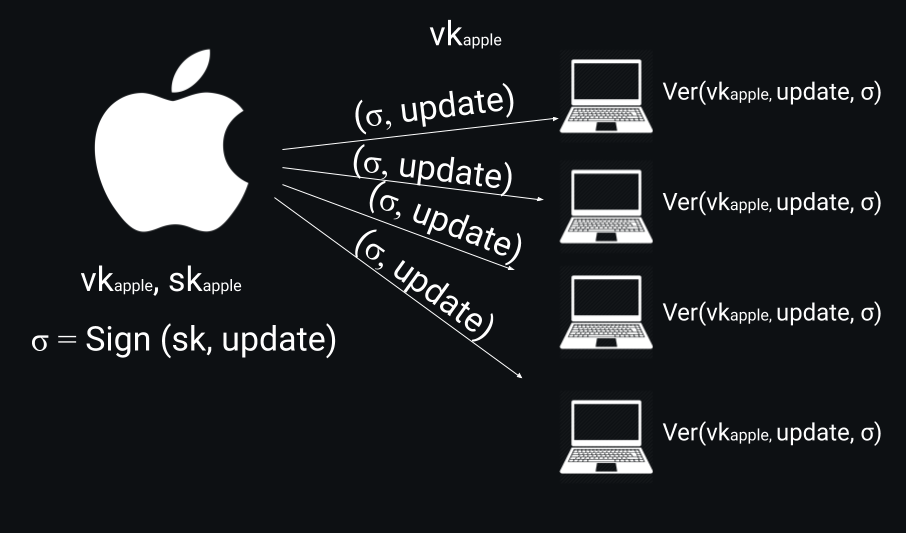
\includegraphics[width=1.1\textwidth]{Signature_software}
\end{figure}
\end{frame}

\begin{frame}{Practical signature schemes}
\Large
\begin{enumerate}
	\itemsep10pt
	\item {\color{Orange} RSA} \\
	-- hardness is based on {\color{Orange} factoring}\\
	-- fast $\Ver$, slow $\Sign, \KeyGen$, much larger keys, signatures	
	\pause
	\item {\color{Orange} (EC)DSA= (Elliptic Curve) Digital Signature Algorithm} \\
	-- hardness is based on {\color{Orange} dlog}\\
	-- slower $\Ver$, fast $\Sign, \KeyGen$\\
	-- for ECDSA much shorter keys, signatures	
	\pause
	\item {\color{Orange} ГОСТ Р 34.10-2012 }  \\
	-- same as ECDSA \\
	-- old ГОСТ Р 34.10-94 was the same as DSA
\end{enumerate}
\pause
\centering

Key sizes (in bits):\\[5pt]
\begin{tabular}{c | c| c}
	Security lvl. & ECDSA / ГОСТ'12 & RSA/DSA \\ \hline
	80 & 160 & 1024 \\
	128 & 256 & 3072 \\
	256 & 512 & 15360
\end{tabular}
\end{frame}

\begin{frame}{Math crash course I: arithmetic in a ring}
\Large 
{\color{Orange} Let $N = p \cdot q$, where $p, q$ are large primes}

\begin{itemize}
	\item $\ZN = \left\{ 0, 1, \ldots, n-1 \right\}$ -- {\color{Orange} ring}
	\item elements in $\ZN$ are added and multiplied modulo $N$, i.e., for $x, y \in \ZN$
	Ex.: $N = 15$
	\begin{align*}
	11+6 \bmod N &= \rem(17, 15) = 2 \\
	6\cdot 7  \bmod N &= \rem(42, 15) = 12
	\end{align*}
	\pause
	\item Not every non-zero $x \in \ZN$ has inverse!
	The set of invertible elements is denoted $\ZN^{\ast} =\{x \in \ZN \; | \;  \gcd(x,N) == 1\}$.\\
	{\large $\gcd $ -- greatest common divisor (НОД)}.\\[5pt]
	Ex.: $3, 6, 9, 5, 10, 12 \notin \ZN^{\ast}$. \\
	$\ZN^{\ast} = \{1, 2, 4, 7, 8, 11, 13, 14\}$.
\end{itemize}

\end{frame}

\begin{frame}{Math crash course I: structure of $\ZN^\ast$ }
\Large 
\begin{itemize}
	\itemsep 10pt
	\item Denote $\phi(N) = |\ZN^\ast|$. $\phi(N)$ is known as {\color{Orange}Euler function} \\
	-- if $N$ -- prime, $\phi(N) = N-1$ (see prev.\ lecture)\\
	-- if $N = p_1^{e_1} \cdot p_n^{e_n}$, $\phi(N)=  N \cdot \prod_{i} \left(1 - \frac{1}{p_i}\right)$. \\
	-- for $N = p \cdot q$, {\color{Orange}$\phi(N) = (p-1)(q-1)$.} \\
	Ex.: $|\ZN^{\ast}| = |\{1, 2, 4, 7, 8, 11, 13, 14\}| = 2 \cdot 4 = 8$.
	\pause
	\item {\color{Orange}Euler's theorem:} for all $a \in \ZN^{\ast}$
	\[
	{\color{Orange}	a^{\phi(n)} = 1 \bmod N }
	\]
	{\large recall Fermat's: $a^{p-1} = 1 \bmod p$ for $p$-prime.}
\end{itemize}
\end{frame}

\begin{frame}{Easy and hard problems in $\ZN$}
\Large 
\begin{center}
{\color{Orange}  $N = p \cdot q$},  $p, q$ are of $\approx$ 1024 bits each.\\
\end{center}
	In $\ZN$ it is  {\color{Orange} easy} to \\[5pt]
	-- add, multiply, find inverse (if exists, or check if does not)\\
	--  compute $g^r \bmod N$ \\[14pt]
	It is {\color{Orange} believed to be  hard} to \\[5pt]
	 -- find $p, q$ \\
	 -- compute square roots in $\ZN$ (as hard as factoring) \\
	 -- compute $e\nth$ roots module $N$ when $\gcd(e, \phi(N)) = 1$\\
	 %-- dlog (TODO)
\end{frame}

\begin{frame}{RSA Key Generation}
\Large
Let $\ell>2$ be an integer and $e>2$ be an odd integer. \\[8pt]
{\color{Orange} $\mathsf{RSAGen}(\ell, e):$}
\begin{enumerate}
	\itemsep5pt
	\item Generate an $\ell$-bit integer $p$ s.t.\ $\gcd(p-1, e)=1$
	\item Generate an $\ell$-bit integer $q \neq p$ s.t.\ $\gcd(q-1, e)=1$
	\item $N= p \cdot q$, $\phi(N) = (p-1)(q-1)$
	\item $d = e^{-1} \bmod \phi(N)$
	\item Output $\vk = (N, e), \sk=(N, d)$
\end{enumerate}
\vspace{10pt}
\large
\pause
\begin{itemize}
	\item there exist efficient probabilistic algorithms to generate primes
	\item Step 4 is correct since $d \in \ZN^\ast$ since \[\gcd(p-1, e) = \gcd(q-1, e) = 1 \implies \gcd((p-1)(q-1), e)=1.\]
	\item there is plenty of conditions on $p,q$ to make the above secure
\end{itemize}
\centering
\Large Do not try to implement $\mathsf{RSAGen}$ yourself. 
\end{frame}

\begin{frame}{RSA Signature Generation and Verification}
\large
$\Hash: \{0,1\}^\ast \rightarrow \ZN^\ast$-- a cryptographic hash-function
\vspace{10pt}
\begin{columns}[t]
	\begin{column}{0.45\textwidth}
		
{\color{Orange} I. $\mathsf{RSASign}(\sk=(N, d), m):$}
\begin{enumerate}
	\itemsep5pt
	\item $y = \Hash(m) \in \ZN^\ast$
	\item $\sigma = y^d \bmod N$
\end{enumerate}
\vspace{10pt}
\pause
{\color{Orange} II. $\mathsf{RSAVerify}(\vk=(N, e), m, \sigma):$}
\begin{enumerate}
	\itemsep5pt
	\item $y' = \sigma^e \bmod N$
	\item $\mathtt{return}(y'==\Hash(m))$ \\
\end{enumerate}
	\end{column}
	\begin{column}{0.55\textwidth}
		\pause
		{\color{Orange} Correctness:}
		For $N=pq$ and $e,d$ s.t.\ $ed = 1 \bmod \phi(N)$ and for all $x \in \Z$
		{\color{Orange} 
		\[
			x^{ed} = x \bmod N
		\] }
	\pause
		Proof: for $k \in \Z$
		\begin{align*}
		&ed = 1 + k \phi(N) = 1+k(p-1)(q-1) \\  \pause
		& x^{p-1} = x \bmod p \quad \text{(Ferma't thm.)}\\ \pause
		& x^{ed} = x^{1+k(p-1)(q-1)} = \\
		& x \cdot (x^{p-1})^{q-1} = x \bmod p \\ \pause
		&\text{Analogously}, x^{ed}  = x \bmod q \\ \pause
		& \implies  p, q \, |\, x^{ed} - x \\
		& \implies   x^{ed} = x \bmod p \cdot q
		\end{align*}
	\end{column}
\end{columns}
\LARGE
\vspace*{-40pt}
{\color{Orange}  $(y^d)^e = y^{ed} = y \bmod N$ } \\[20pt]

\centering
\vfill
Without $\Hash$ the scheme is trivially insecure!
\end{frame}

\begin{frame}{RSA security}
\Large
\begin{itemize}
	\item $\mathsf{RSAGen}(\ell, e) \rightarrow (\vk = (N, e), \sk=(N, d))$
	\item $\mathsf{RSASign}(\sk, m) \rightarrow \sigma = \Hash(m)^e \bmod N$
	\item $\mathsf{RSAVerify}(\vk, m, \sigma) \rightarrow \{0,1\}$
\end{itemize}

{\color{Orange}  RSA Assumption:}
There does not exist a ppt adversary that given $(N, m, m^e)$ for a random $m \in \ZN^\ast$, outputs $m$.\\[10pt]
\pause
{\large Factoring $N \implies $ computing $e\nth$--roots. \\ The inverse is not known! }  \\[10pt]
\pause
{\color{Orange}  Theorem:} The signature scheme ($\mathsf{RSAGen},$ $\mathsf{RSASign},$ $\mathsf{RSAVerify}$) is secure in {\color{Orange}  exsistensial forgery CMA} model under {\color{Orange}  the RSA Assumption} and the assumption that $\Hash$ is a {\color{Orange}  Random Oracle}. \\[10pt]
\pause
Informally, {\color{Orange} a Random Oracle model} is an heuristic way to say that $\Hash$ behaves like a black-box that replies with random (but consistent) outputs.
 
\end{frame}

\begin{frame}{Standards}
\Large 
Variants of RSA Signatures are standardized at PKCS (Public Key Cryptography Standards)  by RSA Security LLC
\url{https://en.wikipedia.org/wiki/PKCS} \\[10pt]

Version 2.2 (latest) of PKCS \#1 includes \\[10pt]
\begin{itemize}
	\itemsep10pt
	\item RSASSA-PSS \\
	SSA = Signature Scheme with Appendix \\
	PSS =  Probabilistic Signature Scheme
	\item  RSASSA-PKCS1-v1\_5 (attacks exist)
\end{itemize}

The standards describe data type conversions, how to represent the data, hash functions, etc.

\end{frame}

\begin{frame}{Usages of signatures schemes}
	\Large
	Practical signature schemes 
	\begin{enumerate}
		\itemsep 10pt
		\item RSA \\
		long keys, signatures; fast verification
		\item ECDSA, GOST\\
		short keys, signatures; slower verification
	\end{enumerate}
\vspace{10pt}
RSA is good for {\color{Orange} Certificates}, ECDSA/GOST are good for e-mails. \\[10pt]

Certificates  bind a public key to an identity.
\end{frame}

\begin{frame}{Certificates and PKI}
\begin{center}
	\begin{tabular}{l c c c l}
		& \Large Alice & &\Large Certificate Authority (CA)&  \\ 
		&  $\pk_{\texttt{A}}$  & & $\vk_{\texttt{CA}}$, $\sk_{\texttt{CA}}$ & \\
		& \multirow{5}{*}{
\includegraphics[scale=0.15]{Alice}} & & &  \\  \pause
		& & $\xrightarrow[\texttt{id, email, } \pk_{\texttt{A}}]{\text {Certificate Signing Request}}$ & & \\  \pause
		& & & Certifying Alice’s identity & \\
		& & & Creating a certificate $\texttt{cert}$& \\
		& & & Signing $\texttt{cert}$& \\
		& & $\xleftarrow{\LARGE \texttt{cert}, \; \sigma = \Sign(\sk_{\texttt{CA}}, \texttt{cert})}$ & & \\  \pause
	\end{tabular}
\end{center}

\vspace{15pt}
\Large
Anyone, who needs to communicate securely with Alice, first runs $\Ver(\vk_{\texttt{CA}} \texttt{cert},\sigma )$. If verification passes, $\pk_{\texttt{A}}$ can be used to communicate with Alice.\\[10pt]

Example: X.509 certificate
\end{frame}

\begin{frame}{Certificate chains}
	\Large
	\begin{center}
	
	\begin{align*}
			&{\LARGE \text{Root CAs } \quad \quad\xrightarrow{\hspace{2em}} \quad \quad \text{Intermediate CA}} \\
			&\text{certifies Interm.\ CAs}  \hspace{46pt} \text{certifies clients} 
	\end{align*}
	\end{center}
	\vspace{20pt}
	There are currently thousands of intermediate CAs operating on the Internet \\[10pt]
	To avoid malicious CAs: {\color{Orange} certificate pinning:} \\[7pt]
	\begin{enumerate}
		\item Every browser maintains a pinning database: \\
		($\texttt{domain}$, $\texttt{hash}_0$, $\texttt{hash}_1, \ldots$ )
		\item The data for each record is provided by the domain owner
		\item 	When the browser connects to a domain, domain sends its certificate chain $\texttt{cert}_0, 
		\texttt{cert}_1, \ldots$
		\item The browser computes $\Hash(\texttt{cert}_i)$ and verifies against $\texttt{hash}_i$. 
	\end{enumerate}
	
\end{frame}

\begin{frame}{The last PA}

	\Large
	Task: implement $\KeyGen, \Sign, \Ver$ for RSA and ECDSA. \\[10pt]
	Compare the speed of $\Sign, \Ver$ for 1000 messages (standard comparison)
\end{frame}

\end{document}
